% !TeX root = ../thuthesis-example.tex
\chapter{水密流形三维网格重建}

针对水密流形三维网格重建问题,本章通过将神经辐射场、可微光栅化和可微光线追踪结合起来,提出了一种新颖的解决方案。在重建高质量的三维网格几何表征的同时,我们通过可微光线追踪辅助,还原高质量的材质信息。

本章将首先对任务进行准确定义,然后介绍所需使用的材质和光照模型,最后对网络中的所有模块进行逐一介绍。

\section{问题描述}

\subsection{水密流形三维网格}

我们要求还原水密流形三维网格的几何表示,这是因为相比于密度场或是其他一些三维网格表示,这样性质良好的表示更有利于后续下游任务的进行。

\textbf{三维网格 (mesh):} 三维网格是由一系列连接的顶点、边和面构成的结构,在计算机图形学和几何建模中用于描述三维对象的形状和结构。在本工作中,我们使用三角形网格,即每个面都是一个三角形。

\textbf{水密 (watertight):} 在三维网格的每条边精确地被两个面共享且不超过两个面的情况下,该网格被称为水密的。

\textbf{流形 (manifold):} 一个流形网格需满足以下条件:(1)每条边连接的面最多为两个;(2)每条边与一个或两个面相交,与一个顶点相连的面以封闭或开放扇形结构组织;(3)面之间禁止相互自相交。图 \ref{fig:nonmanifold} 展示了非流形网格的例子。

\begin{figure}
  \centering
  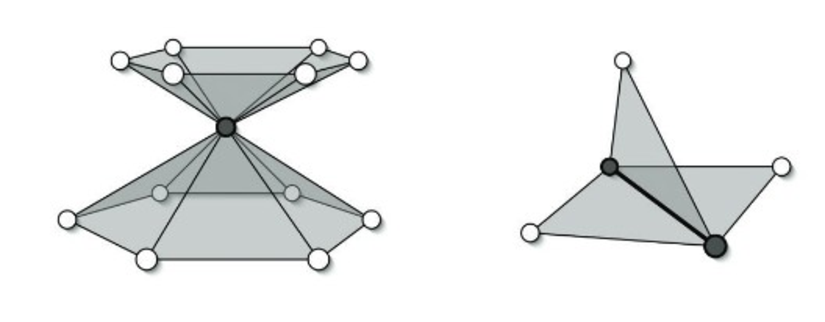
\includegraphics[width=0.8\linewidth]{nonmanifold.pdf}
  \caption{非流形网格示例}
  \label{fig:nonmanifold}
\end{figure}

\subsection{输入}

如上文所述,我们的任务是三维物体的逆渲染。在这个问题中,输入是一系列不同角度所拍摄或渲染的物体图像 $I_1, I_2, \cdots, I_n$,以及相对应的相机位姿参数 $p_1, p_2, \cdots, p_n$。所有图像都是通过相同的相机对同一个物体在固定光照条件下从不同角度进行拍照得到的。我们使用仿真数据来验证我们方法的有效性。

\subsection{输出}
我们模型的输出包含三个部分 $(G, M, L)$。其中 $G$ 代表重建的水密流形三维网格表示,$M$ 代表对应的材质信息,$L$ 则代表光照。

\section{简化的迪士尼原理化BRDF}

我们的模型采用简化的迪士尼原理化BRDF作为着色模型。迪士尼原理化BRDF (Disney Principled BRDF) \cite{DisneyBRDF} 是计算机图形学领域广泛应用的经典着色模型。着色模型的建立是为了准确模拟光照和不同物体表面交互时的不同表现。迪士尼原理化BRDF通过十个参数,能够定义大部分常用表面材质,并且创建逼真且一致的渲染效果。

为了理解着色模型,我们首先需要理解渲染方程:
\begin{equation}
  L_{o}\left(\mathbf{x},\omega_{o}\right) =L_{e}\left(\mathbf{x},\omega_{{o}}\right) +\int_{\Omega}f\left(\mathbf{x},\omega_{{i}},\omega_{{o}}\right)L_{i}\left(\mathbf{x},\omega_{{i}}\right)\cos\theta_{i}d\omega_{{i}},
\end{equation}

其中,$\mathbf{x}$ 指三维空间中的位置,$\omega_i$ 指光线入射方向,$\omega_o$ 指观察方向,$L_o$ 指观察方向的辐射度,$L_e$ 指自发光辐射度,$f$ 指BRDF,$L_i$ 指入射方向的辐射度,$\theta_i$ 指入射方向与法向的夹角。积分域 $\Omega$ 一般是表面法线所对应的半球。我们所说的着色模型主要就是上式中的 $f$ 函数,它接收入射方向和出射方向,返回对应的反射率。

迪士尼原理化BRDF的参数包括漫反射颜色(baseColor)、次表面(subsurface)、金属度(metallic)、高光度(specular)、粗糙度(roughness)、各向异性度(anisotropic)等,其中大部分参数是为了某些特定的材质服务,例如专门为了模仿一些纺织物布料而设计的 sheen 参数。在我们的模型中,为了简便,对迪士尼原理化BRDF做了一些简化,仅保留三项参数:漫反射颜色(baseColor)、粗糙度(roughness)、金属度(metallic)。其中漫反射颜色决定了材质的底色,其余两项参数对物体材质的影响如图\ref{fig:brdf}。
\begin{figure}
  \centering
  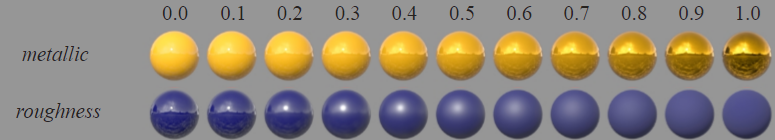
\includegraphics[width=\linewidth]{brdf.png}
  \caption{迪士尼原理化BRDF的两个参数对物体材质的影响}
  \label{fig:brdf}
\end{figure}

\newpage
简化后的 BRDF 函数可以分为漫反射和金属反射两部分。漫反射的BRDF计算公式如下:
\begin{equation}
  f_{\text{Diffuse}} = \frac{\text{baseColor}}{\pi}F_{D}(\omega_{\text{in}})F_{D}(\omega_{\text{out}})|n\cdot\omega_{\text{out}}|,
\end{equation}
其中
\begin{align}
  F_{D}(\omega) &=\begin{pmatrix}1+(F_{D90}-1)(1-|n\cdot\omega|)^5\end{pmatrix}, \\
  F_{D90} &=\frac12+2\cdot\mathrm{roughness}\cdot|h\cdot\omega_{\mathrm{out}}|^2.
\end{align}
金属反射部分的BRDF计算公式如下:
\begin{equation}
  f_\mathrm{metal}=\frac{F_mD_mG_m}{4|n\cdot\omega_\mathrm{in}|},
\end{equation}

其中
\begin{align}
  F_{m} &= C_0+\left(1-C_0\right)\left(1-(h\cdot\omega_{\mathrm{out}})\right)^5,\\
D_{m} &= \frac {\alpha ^ 2} {\pi \left(\mathrm{NoH}^2 (\alpha^2 - 1) + 1\right)^2}, \\
G_{m} &= G(\omega_{in}) G(\omega_{out}),\\
C_0 &= \mathrm{metallic}\cdot\mathrm{baseColor},\\
\alpha &= \max (\mathrm{roughness}^2, 0.0001),\\
\mathrm{NoH}&= \cos (\left<h, n\right>) = h \cdot n,\\
G(\omega) &= \frac 2 {\sqrt{\frac {\alpha^2} {(\omega \cdot n)^2} + 1 - \alpha^2 }+1}.
\end{align}

我们将上述两个部分综合起来得到最终的 BRDF 函数表达式:
\begin{equation}
  f_{\mathrm{final}}=(1-\text{metallic})\cdot f_\text{diffuse}+f_\text{metal}.
\end{equation}

\section{模型设计}

我们的模型流程如图\ref{fig:pipeline}。首先,我们会通过修改版的 TensoIR\cite{tensoir} 得到一个密度场和对应的材质、光照等信息。其次,我们会通过可微 Marching Cube 将三维密度场转换成三维网格表示,同时通过可微光栅化重新优化材质、光照信息,以使其与三维网格表示相匹配。最后,我们通过可微光线追踪技术,固定三维网格表示,优化材质、光照信息,以去除重建的材质中的照明伪影,从而得到更真实的纹理和材质信息。下面我们将对三个部分逐一进行介绍。

\begin{figure}
  \centering
  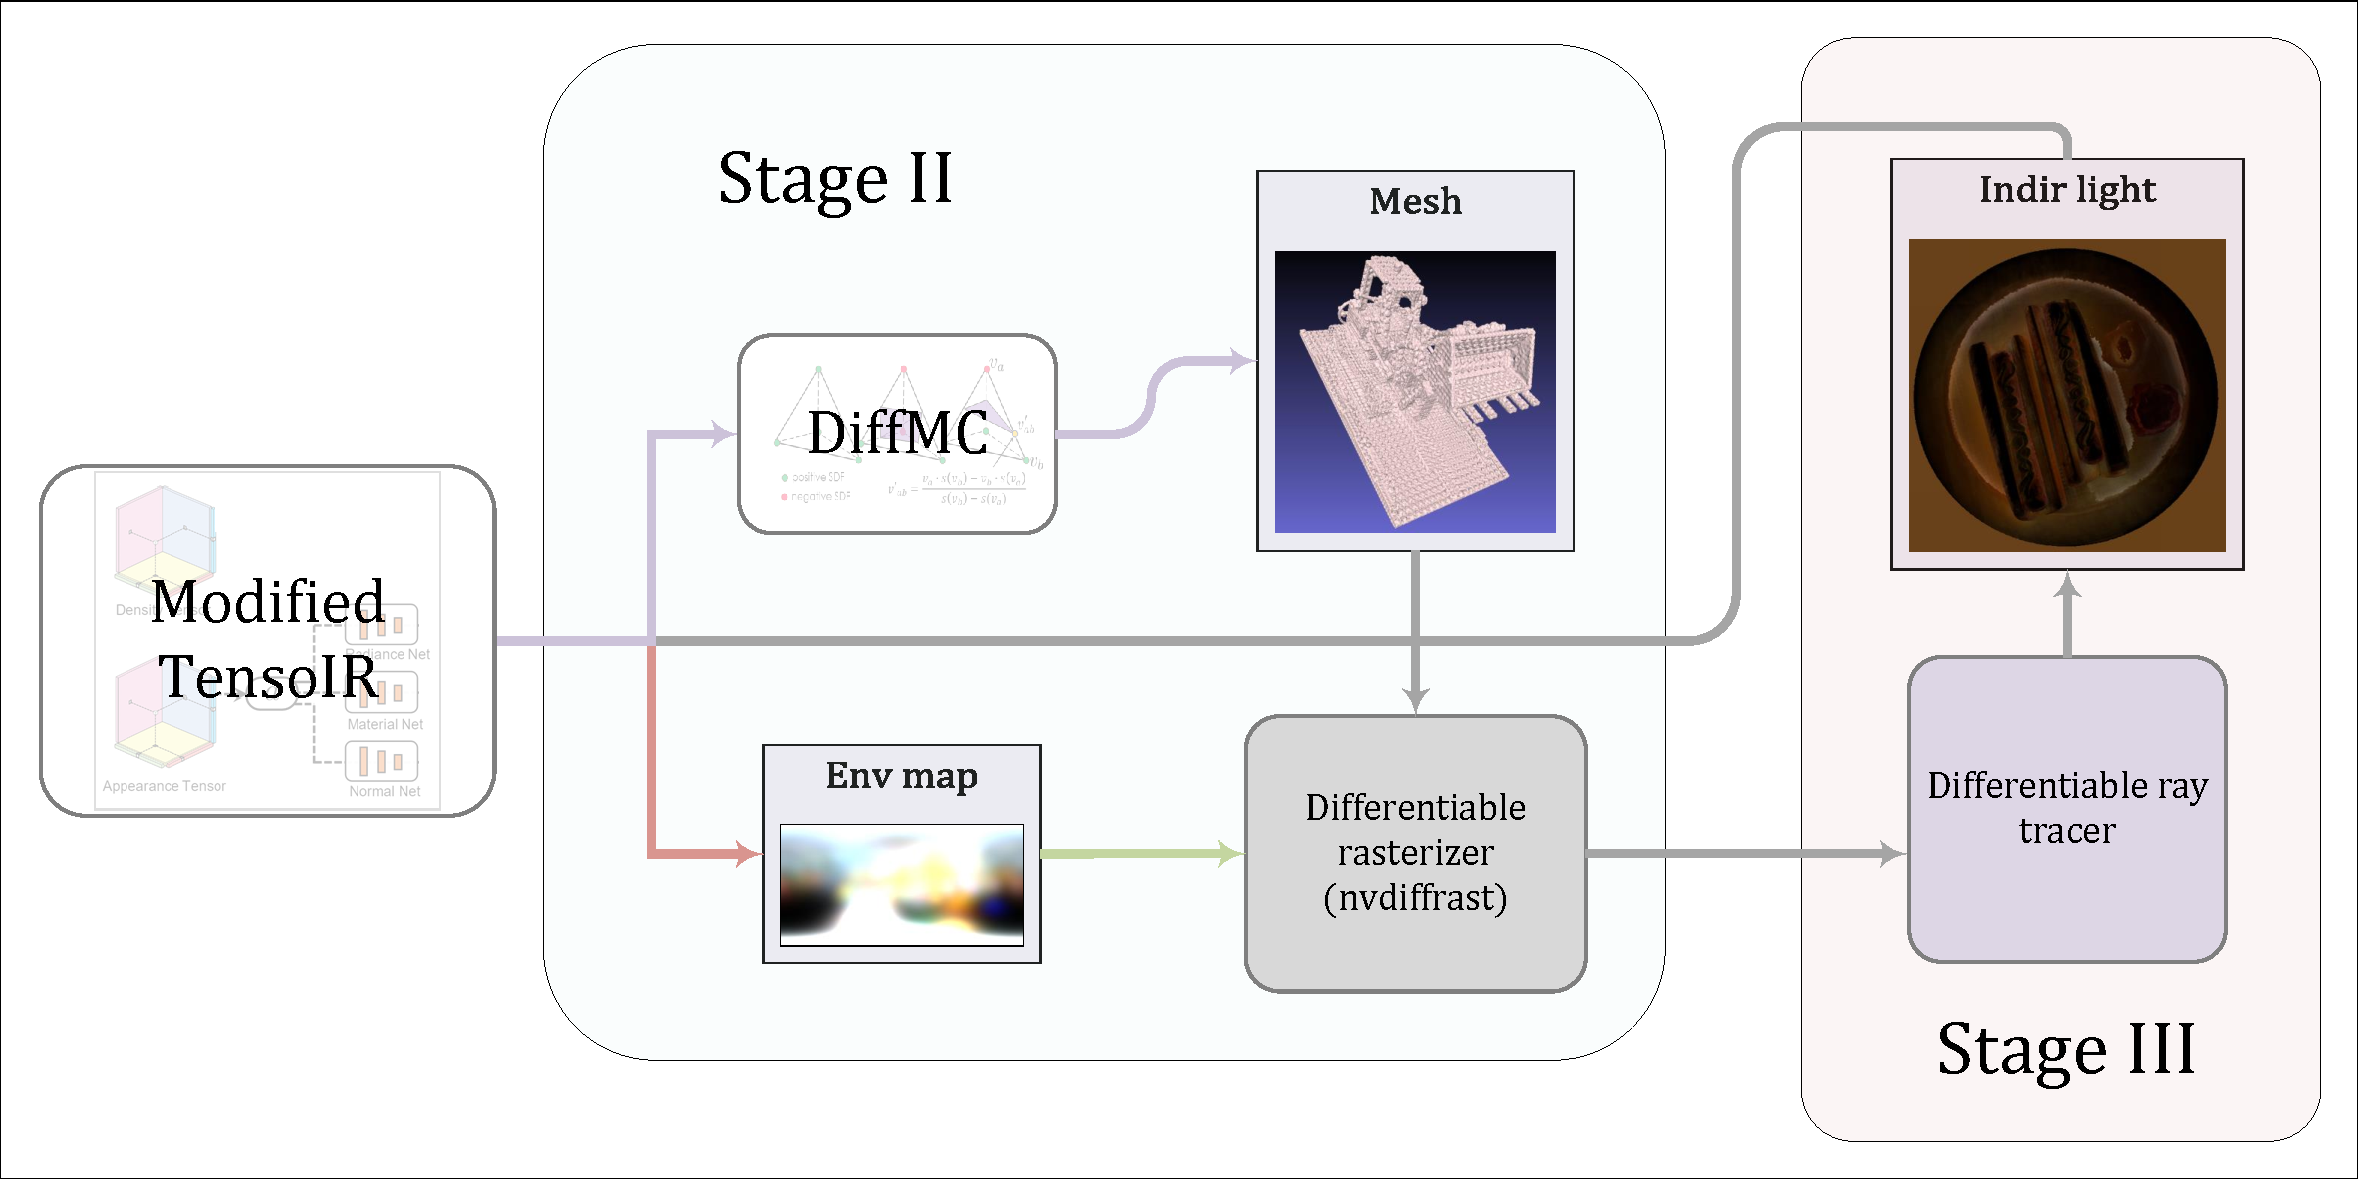
\includegraphics[width=0.7\linewidth]{pipeline.pdf}
  \caption{模型分阶段流程图}
  \label{fig:pipeline}
\end{figure}

\subsection{第一阶段:修改版 TensoIR}

TensoIR 是一个基于神经网络和深度学习的逆渲染框架,由金和刘等人在2022年提出 \cite{tensoir}。该模型在合成和真实数据上都取得了当时的最好效果。它的核心思想在于用 NeRF 中体渲染的方式模拟间接光照,并以此替代路径追踪中的多次迭代,从而实现快速的优化材质信息。它的输入是一系列不同角度所拍摄或渲染的物体图像 $I_1, I_2, \cdots, I_n$,以及相对应的相机位姿参数 $p_1, p_2, \cdots, p_n$。在 TensoIR 中,我们需要同时优化密度场 $D$、外观网络 $a$ 以及环境光照 $L$。TensoIR 的流程如图\ref{fig:tensoir}所示。

TensoIR 的场表示借助了 TensoRF \cite{tensorf} 的表示形式,我们以密度场为例来说明这个表示形式。密度场可以视作函数 $D: \mathrm{R} ^3 \to \mathrm{R}$,输入是三维空间中的位置,输出是一个实数代表密度值。除了用神经网络模拟该函数之外,我们也可以用传统的方式,在三维空间中离散采样,并通过插值计算出任意位置的密度值。假设我们在 $[-1,1]^3$ 的立方体内做均匀采样,我们需要 $O(n^3)$ 的采样点数($n$ 为每个坐标轴上的采样数),这会耗费太多的空间。因此在 TensoRF 中,作者提出了 VM 分解和 CP 分解来解决这个问题。VM 分解是 TensoRF 和 TensoIR 中最终采用的分解方式,因此下面仅对其展开介绍。

\begin{figure}[h]
  \centering
  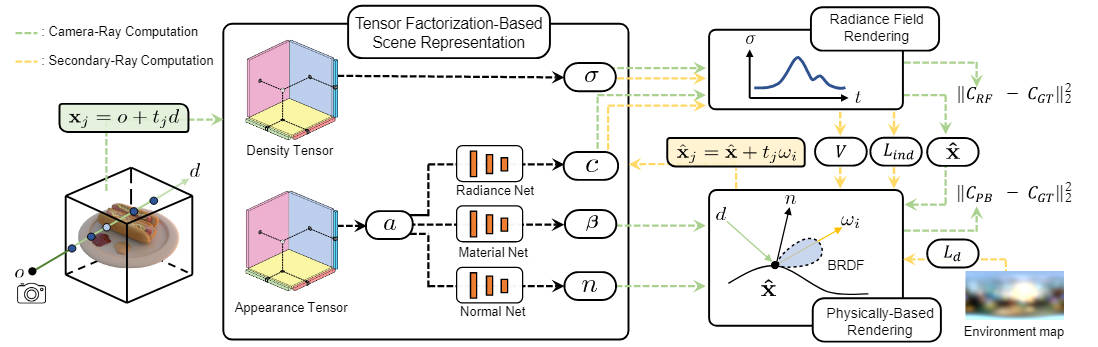
\includegraphics[width=\linewidth]{tensoir.jpg}
  \caption{TensoIR 模型流程图}
  \label{fig:tensoir}
\end{figure}

VM 分解的核心思想在于将三维向量场分解为一维向量和二维矩阵的乘积。具体来说,用 $\mathcal{T}$ 表示三维向量场,我们按照下式进行分解:
\begin{equation}
  \mathcal{T}=\sum_{r=1}^{R_1}\mathbf{v}_r^1\circ\mathbf{M}_r^{2,3}+\sum_{r=1}^{R_2}\mathbf{v}_r^2\circ\mathbf{M}_r^{1,3}+\sum_{r=1}^{R_3}\mathbf{v}_r^3\circ\mathbf{M}_r^{1,2}.
\end{equation}

其中,$\mathbf{v}_r^i$ 是一维向量,$\mathbf{M}_r^{j,k}$ 是一个 $n_j \times n_k$ 的矩阵。这样,我们就将三维向量场分解为了三个部分,每个部分都是一个一维向量和一个二维矩阵的乘积。这样的分解方式使得我们可以用 $O(n^2)$ 的参数量来表示三维向量场。这样分解的坏处在于降低了向量场的表示能力,但是在实际应用中,我们发现 VM 分解的表示能力已经足够应对绝大部分情况。而相较于神经网络,这样的表示方式更为简洁、直接,并且计算效率更高。

如图 \ref{fig:tensoir} 所示,TensoIR 通过上述的表示方式,同时表征密度 $\sigma$,颜色 $c$,BRDF 参数 $\beta$ 和法向方向 $n$。其中,BRDF 参数 $\beta$ 包含两部分,分别是漫反射率 $\alpha = \mathrm{MLP}_{\mathrm{albedo}}(\beta)$ 以及表面粗糙度 $r=\mathrm{MLP}_{\mathrm{roughness}}(\beta)$。根据这些参数,他们得以同时进行神经辐射场渲染和基于物理的渲染,并同时对上述所有参数进行优化。在基于物理的渲染中,他们对渲染方程做出了改动:
\begin{equation}
  L_{\mathrm{i}}(\mathbf{\hat{x}},\omega_{i})=V(\mathbf{\hat{x}},\omega_{i})L_{\mathrm{d}}(\omega_{i})+L_{\mathrm{ind}}(\mathbf{\hat{x}},\omega_{i}),
\end{equation}
其中 $V$ 是可见性函数,$L_{\mathrm{d}}$ 是直接光照,$L_{\mathrm{ind}}$ 是间接光照。我们用神经辐射场模拟间接光照,即:
\begin{equation}
  L_{\mathrm{ind}}(\mathbf{\hat{x}},\omega_i)=C_{\mathrm{RF}}(\mathbf{\hat{x}},\omega_i).
\end{equation}

在我们的模型中,由于所需参数不同,我们对 BRDF 参数 $\beta$ 做了一些改动。在 3.2 节中提到,我们的着色模型需要漫反射颜色(baseColor)、粗糙度(roughness)、金属度(metallic)三个参数。因此我们通过三个不同的多层感知机来分别预测这三个参数,并根据这些参数进行着色和基于物理的渲染。

关于环境光照,我们假设其为一个球形高斯混合模型,即 $L(\omega) = \sum_{i=1}^k w_i \mathcal{N}(\mu_i, \Sigma_i)$,其中 $\omega$ 是光线的方向,$w_i$ 是权重,$\mu_i$ 是均值,$\Sigma_i$ 是协方差矩阵。后续的可微光栅化和可微光线追踪也都会使用这个光照模型。

由于 TensoIR 同时通过神经辐射场和物理模型渲染两张图片,与真实图像计算损失函数,并同时优化上述提及的所有参数,它能够提供较为精确的密度场、材质信息和光照信息,可以给后续训练一个很好的初始化。在第一阶段结束后,我们获得了一个较为精准的密度场 $\sigma$,BRDF 参数 $\beta$,法向方向 $n$ 和用球形高斯表示的环境光 $L$。

\subsection{第二阶段:可微光栅化}

在第二阶段中,我们首先通过可微 Marching Cube 将三维密度场转换成三维网格表示,并通过可微光栅化,在一阶段结果的基础上,同时优化几何形状、材质、光照信息。

\subsubsection{可微 Marching Cube (DiffMC) \cite{wei2023neumanifold}}

我们首先通过可微 Marching Cube 将三维密度场 $\sigma$ 可微地转化成三维网格表示。Marching Cube 是一种常用的三维重建算法,然而,传统的 Marching Cube 算法 \cite{MarchingCube} 是不可微的,这使得我们无法直接在神经网络中使用并反向传播梯度。因此,我们需要对 Marching Cube 算法进行改进,使其可微。这里我们直接使用了 Wei 等人实现的可微 Marching Cube 模块。该模块接受有符号距离场作为输入,通过一个可微的前向过程,生成一个水密流形三维网格。在训练过程中,我们可以直接对有符号距离场进行反向传播,从而优化几何形状。

但是在第一阶段中获得的密度场 $\sigma$ 并不能直接作为 DiffMC 的输入,因此我们需要首先将其转换为有符号距离场。我们首先将密度转换为不透明度:
\begin{equation}
  \alpha = 1 - \exp(-\sigma \cdot \delta).
\end{equation}

其中,$\alpha$ 表示不透明度,$\sigma$ 表示密度值,$\delta$ 表示第一阶段 TensoIR 中使用的体渲染的步长。我们设定 $t$ 为一个阈值,当 $\alpha > t$ 时,我们认为该点在物体内部,当 $\alpha \leq t$ 时,我们认为该点在物体外部。我们将有符号距离场定义为:
\begin{equation}
  \text{SDF} = \alpha - t.
\end{equation}

我们将该 $\text{SDF}$ 作为 DiffMC 的输入,并以此得到水密流形三维网格表示 $G$。

\subsubsection{可微光栅化}

在得到三维网格表示 $G$ 后,我们需要将其与 BRDF 参数 $\beta$ 和环境光 $L$ 相结合,渲染出图像,并与真实图像计算损失。

在3.3.2.1 节可微 Marching Cube 中,我们将密度场转换为三维网格表示。这一步骤同样带来了问题。原先的材质信息 $\beta$ 是与密度场 $\sigma$ 和体渲染相对应,但在3.3.2节中,我们需要与新的三维网格表示 $G$ 与光栅化相结合,因此需要重新优化材质信息。但原先的材质信息提供了一个很好的初始化。这是因为如果给定一个准确的密度场 $\sigma^*$ (物体外部密度为 $0$,物体内部密度为$1$)和对应的准确的三维网格表示 $G$,那么通过体渲染和光栅化分别得到的两组渲染图像几乎是相同的。因此,可微 Marching Cube 带来的表示形式的迁移造成的误差本质上是由于密度场的不准确性造成的。而 TensoIR 提供的密度场的误差相对较小,因而我们可以用3.3.1节得到的 BRDF 参数 $\beta$ 作为初始化,通过优化得到更好的材质信息。

我们使用 nvdiffrast \cite{nvdiffrast} 作为可微光栅化器。在渲染时,我们计算各个方向光线与三维网格的表面交点,并用表面法向网络 $n$ 而非根据 $G$ 计算的法向 $n'$ 作为法向信息进行渲染,这是因为 $n'$ 同时也受到密度场不准确的影响。

在这一阶段训练结束后,我们期望得到一组三维网格表示 $G$,以及与之对应的 BRDF 参数 $\beta$,法向网络 $n$以及环境光照 $L$。在这一步结束后我们已经可以导出一个高质量的三维网格表示。但是,由于我们使用的 TensoIR 中的体渲染和第二阶段的可微光栅化都不能很好地处理全局光照,这一步结束后材质中会存在大量照明伪影。因此,我们需要引入第三阶段,通过可微光线追踪来解决这个问题。

\begin{figure}
  \centering
  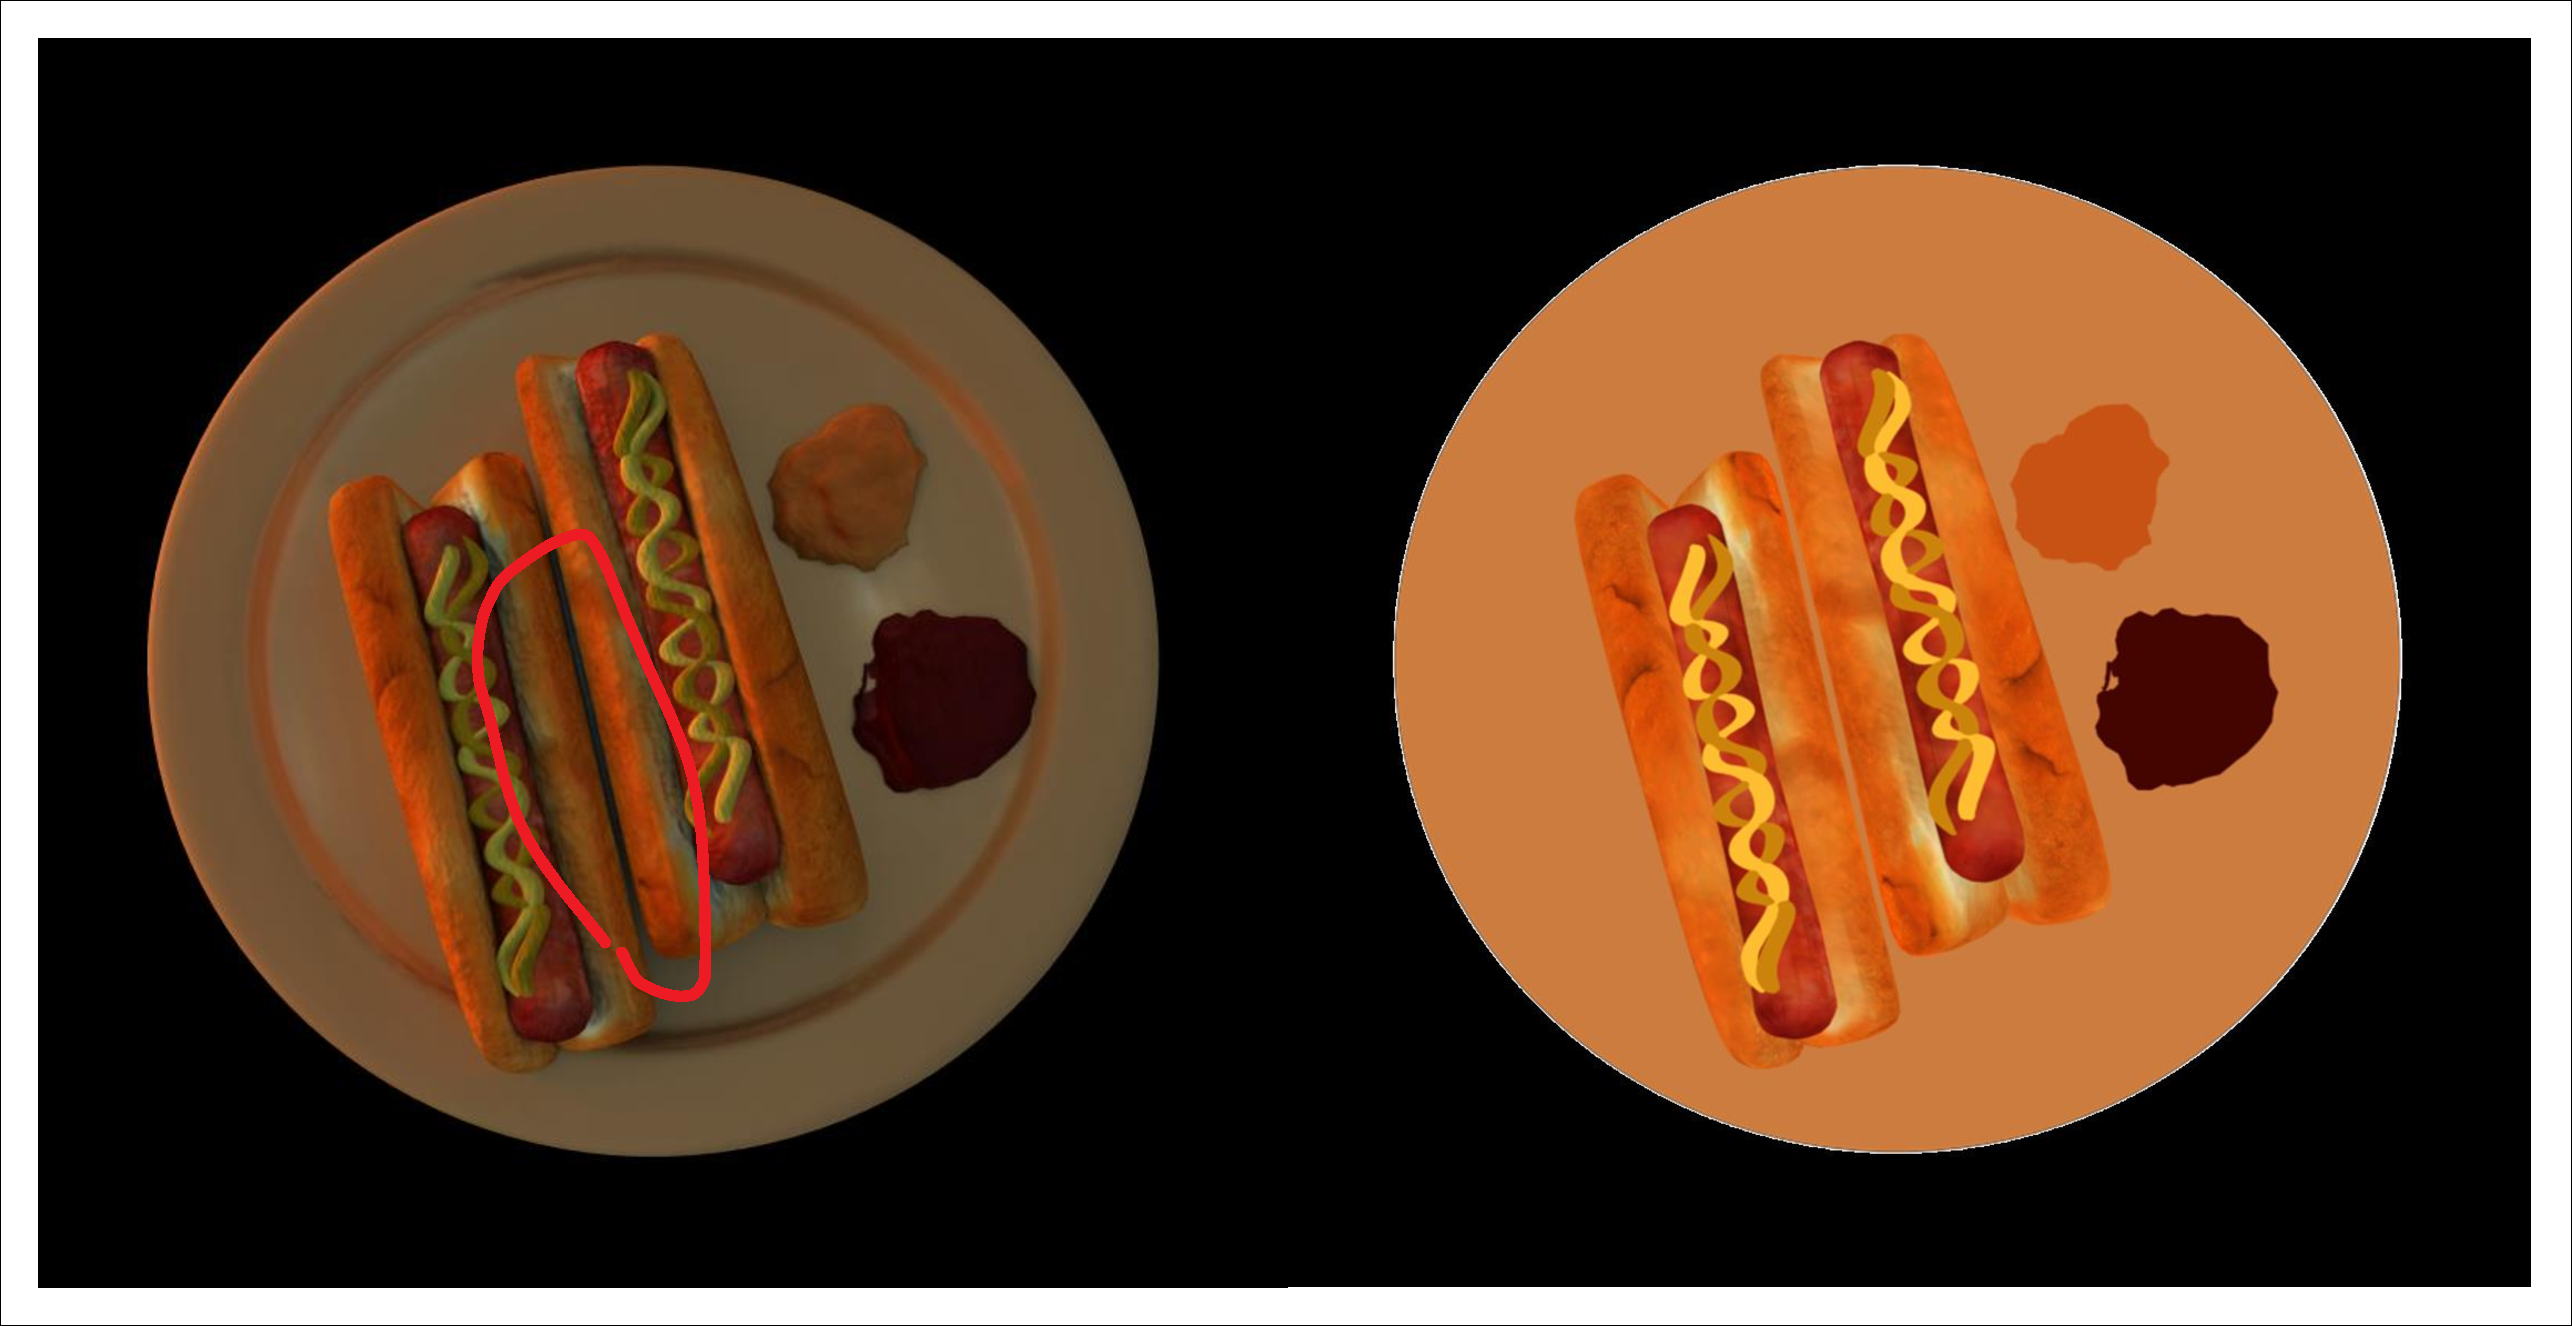
\includegraphics[width=\linewidth]{bakedshadow.pdf}
  \caption{材质中的照明伪影示意}
  \label{fig:bakedshadow}
\end{figure}

如图 \ref{fig:bakedshadow}。左侧是第二阶段训练结束后生成的漫反射颜色图像,右侧是真实的漫反射颜色图像。可以看到,左侧图像红圈内的区域存在照明伪影,呈黑色,这是因为我们的模型无法很好地处理全局光照,因此错误地将阴影所产生的黑色烘焙进材质里。而右侧图像对应位置的颜色与盘子的底色是完全相同的,并没有阴影出现。

\subsection{第三阶段:可微光线追踪}

在第二阶段,我们已经生成了水密流形三维网格 $G$,以及对应的 BRDF 参数 $\beta$,环境光照 $L$。接下来我们引入可微光线追踪来减少材质中的照明伪影。

\subsubsection{原理}

在 2.2.2 节,我们对可微光线追踪进行了介绍,也提到了它的优缺点。我们提到,由于可微光线追踪考虑了全局光照,能够真实准确地模拟光线与物体表面的交互过程。然而,由于计算几何形状梯度的困难性,现有的可微光线追踪方法往往效率低下,渲染一张图片并计算梯度的时间成本很高,不适用于神经网络训练。我们调研了现有的可微光线追踪方法,但都不适合我们的使用场景。具体分析可见附录 \ref{sec:compare}。

注意到,我们已经通过可微 Marching Cube 得到了一个高质量三维网格表示 $G$,因而我们可以固定三维几何表示,优化其余参数。这样,我们也不需要计算最终损失函数关于几何形状的梯度,从而大大简化可微光线追踪。虽然光线追踪中涉及大量的随机采样过程,但在固定几何表示 $G$ 的情况下,从相机位置出发的每一条光路在计算渲染前都是已经确定的。我们只需要根据采样得到的光路,计算每条光路与物体表面交互的过程,并得到渲染图像,整个过程自然是可微的。

\subsubsection{实现}

根据上述原理,我们自己实现了可微光线追踪框架。接下来我们将简要介绍实现细节。

我们的可微光线追踪器 new-renderer,接受场景信息(包括多个物体、对应的材质和环境光照)及光线方向作为输入,输出渲染后的图像。在渲染过程中,由于硬件限制,我们设定每像素采样率 $\text{spp}=128$,光线追踪深度 $\text{depth}=6$。

我们仿照 Mitsuba 的格式用字典储存整个场景。场景中的每个物体都保存为单独的 obj 文件,并在场景字典中通过 to\_world 矩阵指定其在场景中的位置。

我们仿照 pbrt \cite{PBRT3e} 的方式实现渲染器。除了我们模型中需要用到的神经网络材质模型外,为了调试渲染器以及确定渲染器的正确性,我们也实现了额外的材质模型,包括漫反射模型、简化版原理化 BRDF 模型、导体 BRDF。所有的材质模型都封装成统一格式的类,并且提供计算反射率函数值、重要性采样以及计算采样概率的借口。我们也实现了额外的光照模型,包括点光源模型和纯色环境光模型。

我们借助 Mitsuba\cite{Mitsuba3} 库计算光线与物体表面的交点。在后续工作中,我们也考虑自行实现光线与物体表面的交点计算,以减少依赖并提升效率。在这一阶段,我们仍然使用法向网络 $n$ 而非几何形状 $G$ 计算得到的法向作为法向信息进行渲染。这不仅省去了计算几何形状梯度的步骤,保持模型统一性,而且神经网络表示的法向场可以让渲染结果更平滑,不再需要抗锯齿或法线插值等操作。

在第三阶段完成后,我们已经得到了一个高质量的三维网格表示 $G$,以及对应的 BRDF 参数 $\beta$,法向网络 $n$ 和环境光照 $L$。这一阶段结束后,我们期望从材质中去除了部分照明伪影,还原了更真实的漫反射颜色。

\section{训练方法}

最朴素的训练方法是按照阶段顺序依次训练。此外,我们也支持第二、第三阶段的反复训练。第三阶段的目的是去除烘焙在材质中的照明伪影,我们在训练过程中固定了三维几何表示,优化剩余参数。事实上,几何表示的质量和光线追踪的效果息息相关。几何表示与真实几何的差异会导致光线追踪光路的误差,而这种差异在反射次数增加时会被放大。因此,我们也需要在可微光线追踪结束后,通过重新进行可微光栅化训练更新三维网格表示 $G$。反复的迭代可以带来更高质量的重建和逆渲染结果。
